\section{B--Spline Fitting}
\newcommand{\norm}[1]{\parallel #1 \parallel_2}

\subsection{Current Status}
\begin{frame}{Current status}
\begin{minipage}[t]{0.4\linewidth}

\begin{itemize}
\item What do we have so far?
\end{itemize}
\vspace{5mm}
\begin{figure}
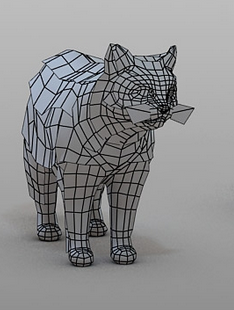
\includegraphics[width=0.8\linewidth]{Pictures/cat.png}
\end{figure}
\end{minipage}%
%\hfill%
\pause
\begin{minipage}[t]{0.6\linewidth}
\begin{itemize}
\item What if we try to pass it to an engineer?
\end{itemize}

\begin{figure}

\includegraphics[width=0.9\linewidth]{Pictures/engineerThoughts2.png}
\end{figure}
\vspace{5mm}
\end{minipage}

\textbf{How to make CAD understand our data?}
\end{frame}

\subsection{B--Spline}
\begin{frame}{B--Spline}
\begin{equation*}
\vec{S}\left(u,v\right)=\sum\limits_{i,j=1}^{n,m} \vec{C}_{i,j} N_i^p\left(u\right) N_j^p\left(v\right),
\end{equation*}
where $p$ -- degree of the B--Spline surface and $n,m$ -- number of control points in each direction.
\begin{columns}
\begin{column}{.45\textwidth}
B--Splines
\begin{itemize}
\item offer great flexibility for handling arbitrary shapes
\item are CAD--standard
\end{itemize}
\textbf{Engineers are working with CAD}
\end{column}
\begin{column}{.45\textwidth}
% This file was created by matlab2tikz.
% Minimal pgfplots version: 1.3
%
%The latest updates can be retrieved from
%  http://www.mathworks.com/matlabcentral/fileexchange/22022-matlab2tikz
%where you can also make suggestions and rate matlab2tikz.
%
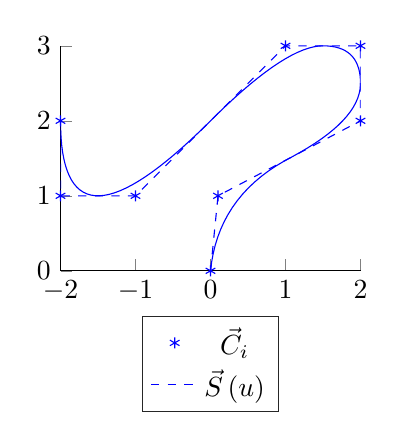
\begin{tikzpicture}

\begin{axis}[%
width=1.5in,
height=1.125in,
scale only axis,
xmin=-2,
xmax=2,
ymin=0,
ymax=3,
axis x line*=bottom,
axis y line*=left,
legend style={at={(.5,-.2)},anchor = north,draw=white!15!black}
]
\addplot [color=blue,only marks,mark=asterisk,mark options={solid}]
  table[row sep=crcr]{%
0	0\\
0.1	1\\
2	2\\
2	3\\
1	3\\
-1	1\\
-2	1\\
-2	2\\
};
\addlegendentry{$\vec{C}_i$};

\addplot [color=blue,dashed]
  table[row sep=crcr]{%
0	0\\
0.1	1\\
2	2\\
2	3\\
1	3\\
-1	1\\
-2	1\\
-2	2\\
};

\addplot [color=blue,solid]
  table[row sep=crcr]{%
0	0\\
0.01506	0.1182\\
0.03624	0.2328\\
0.06354	0.3438\\
0.09696	0.4512\\
0.1365	0.555\\
0.18216	0.6552\\
0.23394	0.7518\\
0.29184	0.8448\\
0.35586	0.9342\\
0.426	1.02\\
0.50226	1.1022\\
0.58464	1.1808\\
0.67314	1.2558\\
0.76776	1.3272\\
0.8685	1.395\\
0.97536	1.4592\\
1.08762	1.52\\
1.19592	1.58\\
1.29738	1.64\\
1.392	1.7\\
1.47978	1.76\\
1.56072	1.82\\
1.63482	1.88\\
1.70208	1.94\\
1.7625	2\\
1.81608	2.06\\
1.86282	2.12\\
1.90272	2.18\\
1.93578	2.24\\
1.962	2.3\\
1.98138	2.36\\
1.99392	2.42\\
1.99962	2.48\\
1.9992	2.5392\\
1.995	2.595\\
1.9872	2.6472\\
1.9758	2.6958\\
1.9608	2.7408\\
1.9422	2.7822\\
1.92	2.82\\
1.8942	2.8542\\
1.8648	2.8848\\
1.8318	2.9118\\
1.7952	2.9352\\
1.755	2.955\\
1.7112	2.9712\\
1.6638	2.9838\\
1.6128	2.9928\\
1.5582	2.9982\\
1.5	3\\
1.4382	2.9964\\
1.3728	2.9856\\
1.3038	2.9676\\
1.2312	2.9424\\
1.155	2.91\\
1.0752	2.8704\\
0.991799999999999	2.8236\\
0.904799999999999	2.7696\\
0.8142	2.7084\\
0.72	2.64\\
0.6222	2.5644\\
0.5208	2.4816\\
0.4158	2.3916\\
0.3072	2.2944\\
0.195000000000001	2.19\\
0.0792000000000008	2.0784\\
-0.0397999999999993	1.9604\\
-0.156799999999999	1.8464\\
-0.270199999999999	1.7396\\
-0.379999999999999	1.64\\
-0.4862	1.5476\\
-0.5888	1.4624\\
-0.6878	1.3844\\
-0.7832	1.3136\\
-0.875	1.25\\
-0.9632	1.1936\\
-1.0478	1.1444\\
-1.1288	1.1024\\
-1.2062	1.0676\\
-1.28	1.04\\
-1.3502	1.0196\\
-1.4168	1.0064\\
-1.4798	1.0004\\
-1.5392	1.0016\\
-1.595	1.01\\
-1.6472	1.0256\\
-1.6958	1.0484\\
-1.7408	1.0784\\
-1.7822	1.1156\\
-1.82	1.16\\
-1.8542	1.2116\\
-1.8848	1.2704\\
-1.9118	1.3364\\
-1.9352	1.4096\\
-1.955	1.49\\
-1.9712	1.5776\\
-1.9838	1.6724\\
-1.9928	1.7744\\
-1.9982	1.8836\\
-2	2\\
};
\addlegendentry{$\vec{S}\left(u\right)$};

\end{axis}
\end{tikzpicture}%
\end{column}
\end{columns}
\end{frame}

\begin{frame}{B--Spline Fitting}
\only<1>{
% This file was created by matlab2tikz.
% Minimal pgfplots version: 1.3
%
%The latest updates can be retrieved from
%  http://www.mathworks.com/matlabcentral/fileexchange/22022-matlab2tikz
%where you can also make suggestions and rate matlab2tikz.
%
\begin{tikzpicture}

\begin{axis}[%
width=3.5in,
height=1.5in,
scale only axis,
xmin=-1,
xmax=7,
ymin=-1,
ymax=1,
axis x line*=bottom,
axis y line*=left,
legend style={legend columns=-1,at={(.5,-.15)},draw=white!15!black,anchor=north}
]
\addplot [color=red,only marks,mark=asterisk,mark options={solid}]
  table[row sep=crcr]{%
0	0\\
0.15707963267949	0.453990499739547\\
0.314159265358979	0.809016994374947\\
0.471238898038469	0.987688340595138\\
0.628318530717959	0.951056516295154\\
0.785398163397448	0.707106781186548\\
0.942477796076938	0.309016994374948\\
1.09955742875643	-0.156434465040231\\
1.25663706143592	-0.587785252292473\\
1.41371669411541	-0.891006524188368\\
1.5707963267949	-1\\
1.72787595947439	-0.891006524188368\\
1.88495559215388	-0.587785252292473\\
2.04203522483337	-0.156434465040231\\
2.19911485751286	0.309016994374947\\
2.35619449019234	0.707106781186547\\
2.51327412287183	0.951056516295154\\
2.67035375555132	0.987688340595138\\
2.82743338823081	0.809016994374948\\
2.9845130209103	0.453990499739546\\
3.14159265358979	3.67394039744206e-16\\
3.29867228626928	-0.453990499739546\\
3.45575191894877	-0.809016994374947\\
3.61283155162826	-0.987688340595138\\
3.76991118430775	-0.951056516295154\\
3.92699081698724	-0.707106781186548\\
4.08407044966673	-0.309016994374948\\
4.24115008234622	0.156434465040231\\
4.39822971502571	0.587785252292473\\
4.5553093477052	0.891006524188367\\
4.71238898038469	1\\
4.86946861306418	0.891006524188368\\
5.02654824574367	0.587785252292474\\
5.18362787842316	0.156434465040232\\
5.34070751110265	-0.309016994374945\\
5.49778714378214	-0.707106781186548\\
5.65486677646163	-0.951056516295153\\
5.81194640914112	-0.987688340595138\\
5.96902604182061	-0.809016994374947\\
6.1261056745001	-0.453990499739547\\
6.28318530717959	-7.34788079488412e-16\\
};
\addlegendentry{$\vec{P}_\alpha$};

\end{axis}
\end{tikzpicture}%

}
\only<2>{
% This file was created by matlab2tikz.
% Minimal pgfplots version: 1.3
%
%The latest updates can be retrieved from
%  http://www.mathworks.com/matlabcentral/fileexchange/22022-matlab2tikz
%where you can also make suggestions and rate matlab2tikz.
%
\definecolor{mycolor1}{rgb}{0.00000,0.44700,0.74100}%
\definecolor{mycolor2}{rgb}{0.85000,0.32500,0.09800}%
%
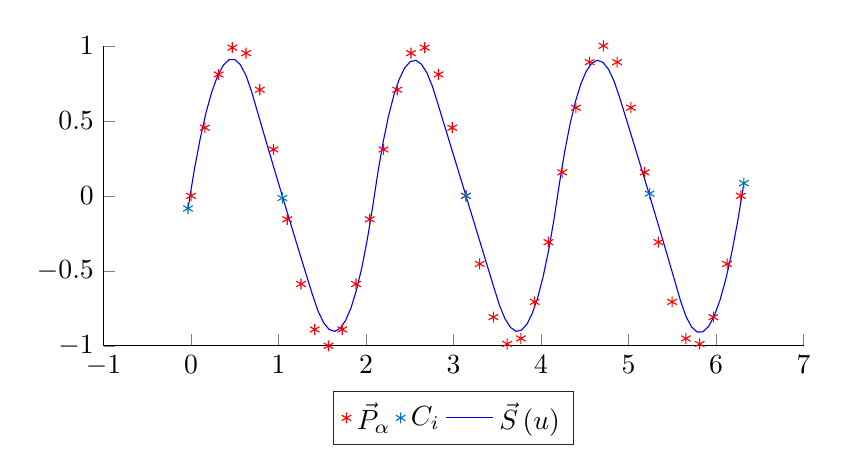
\begin{tikzpicture}

\begin{axis}[%
width=3.5in,
height=1.5in,
scale only axis,
xmin=-1,
xmax=7,
ymin=-1,
ymax=1,
axis x line*=bottom,
axis y line*=left,
legend style={legend columns=-1,at={(.5,-.15)},draw=white!15!black,anchor=north}
]
\addplot [color=red,only marks,mark=asterisk,mark options={solid}]
  table[row sep=crcr]{%
0	0\\
0.15707963267949	0.453990499739547\\
0.314159265358979	0.809016994374947\\
0.471238898038469	0.987688340595138\\
0.628318530717959	0.951056516295154\\
0.785398163397448	0.707106781186548\\
0.942477796076938	0.309016994374948\\
1.09955742875643	-0.156434465040231\\
1.25663706143592	-0.587785252292473\\
1.41371669411541	-0.891006524188368\\
1.5707963267949	-1\\
1.72787595947439	-0.891006524188368\\
1.88495559215388	-0.587785252292473\\
2.04203522483337	-0.156434465040231\\
2.19911485751286	0.309016994374947\\
2.35619449019234	0.707106781186547\\
2.51327412287183	0.951056516295154\\
2.67035375555132	0.987688340595138\\
2.82743338823081	0.809016994374948\\
2.9845130209103	0.453990499739546\\
3.14159265358979	3.67394039744206e-16\\
3.29867228626928	-0.453990499739546\\
3.45575191894877	-0.809016994374947\\
3.61283155162826	-0.987688340595138\\
3.76991118430775	-0.951056516295154\\
3.92699081698724	-0.707106781186548\\
4.08407044966673	-0.309016994374948\\
4.24115008234622	0.156434465040231\\
4.39822971502571	0.587785252292473\\
4.5553093477052	0.891006524188367\\
4.71238898038469	1\\
4.86946861306418	0.891006524188368\\
5.02654824574367	0.587785252292474\\
5.18362787842316	0.156434465040232\\
5.34070751110265	-0.309016994374945\\
5.49778714378214	-0.707106781186548\\
5.65486677646163	-0.951056516295153\\
5.81194640914112	-0.987688340595138\\
5.96902604182061	-0.809016994374947\\
6.1261056745001	-0.453990499739547\\
6.28318530717959	-7.34788079488412e-16\\
};
\addlegendentry{$\vec{P}_\alpha$};

\addplot [color=mycolor1,only marks,mark=asterisk,mark options={solid}]
  table[row sep=crcr]{%
-0.0348836998248783	-0.0846758619167869\\
0.349556990541399	1.38684482775949\\
1.0428028510824	-0.0145597417433248\\
1.75736069888241	-1.35114915293313\\
2.43262150105756	1.35612296417542\\
3.14159265358979	1.01732313646336e-15\\
3.85056380612203	-1.35612296417542\\
4.52582460829717	1.35114915293313\\
5.24038245609718	0.0145597417433281\\
5.93362831663819	-1.38684482775949\\
6.31806900700446	0.0846758619167872\\
};
\addlegendentry{$C_i$};
\addplot [color=blue,solid]
  table[row sep=crcr]{%
-0.0348836998248783	-0.0846758619167869\\
0.0340093005842759	0.162602856132079\\
0.102289653279878	0.374691561995216\\
0.169957358261929	0.551590255672624\\
0.237012415530429	0.693298937164304\\
0.303454825085377	0.799817606470256\\
0.369284586926773	0.871146263590479\\
0.434501701054617	0.907284908524974\\
0.49910616746891	0.90823354127374\\
0.563097986169652	0.873992161836778\\
0.626477157156842	0.804560770214087\\
0.68924368043048	0.699939366405668\\
0.751707788014408	0.574237585954459\\
0.814339675319762	0.448840345230227\\
0.877144189721914	0.32396810728833\\
0.940121331220864	0.199620872128769\\
1.00327109981661	0.0757986397515427\\
1.06659349550916	-0.0474985898433481\\
1.1300885182985	-0.170270816655903\\
1.19375616818464	-0.292518040686123\\
1.25759644516758	-0.414240261934008\\
1.32160934924732	-0.535437480399557\\
1.38579488042386	-0.656109696082771\\
1.45000454656663	-0.766508245377186\\
1.51390802844641	-0.84494732556638\\
1.57749320425663	-0.890631127376358\\
1.64076007399729	-0.90355965080712\\
1.70370863766839	-0.883732895858664\\
1.76633889526993	-0.831150862530991\\
1.82865084680191	-0.745813550824103\\
1.89064449226432	-0.627720960737997\\
1.95231983165718	-0.476873092272674\\
2.01367686498047	-0.293269945428134\\
2.0747155922342	-0.0769115202043776\\
2.13556742673114	0.157609121501347\\
2.19665946173778	0.362864528522984\\
2.25802455058231	0.535206435386219\\
2.31966269326473	0.674634842091055\\
2.38157388978504	0.781149748637492\\
2.44375814014325	0.854751155025527\\
2.50621544433935	0.895439061255163\\
2.56894580237334	0.903213467326397\\
2.63194921424523	0.878074373239233\\
2.695225679955	0.820021778993667\\
2.75877519950267	0.729055684589701\\
2.82255563495029	0.610255333878941\\
2.88636303867819	0.488204267103153\\
2.95017044240609	0.366153200327364\\
3.01397784613399	0.244102133551577\\
3.07778524986189	0.122051066775789\\
3.14159265358979	4.9960036108132e-16\\
3.2054000573177	-0.122051066775788\\
3.2692074610456	-0.244102133551576\\
3.3330148647735	-0.366153200327364\\
3.3968222685014	-0.488204267103153\\
3.4606296722293	-0.610255333878941\\
3.52441010767691	-0.729055684589702\\
3.58795962722458	-0.820021778993668\\
3.65123609293436	-0.878074373239233\\
3.71423950480624	-0.903213467326398\\
3.77696986284024	-0.895439061255163\\
3.83942716703634	-0.854751155025528\\
3.90161141739454	-0.781149748637493\\
3.96352261391486	-0.674634842091057\\
4.02516075659728	-0.53520643538622\\
4.08652584544181	-0.362864528522986\\
4.14761788044845	-0.157609121501349\\
4.20846971494538	0.076911520204376\\
4.26950844219912	0.293269945428133\\
4.33086547552241	0.476873092272673\\
4.39254081491526	0.627720960737995\\
4.45453446037768	0.745813550824102\\
4.51684641190965	0.831150862530991\\
4.57947666951119	0.883732895858664\\
4.64242523318229	0.903559650807119\\
4.70569210292295	0.890631127376359\\
4.76927727873318	0.844947325566381\\
4.83318076061296	0.766508245377186\\
4.89739042675573	0.656109696082772\\
4.96157595793226	0.535437480399558\\
5.025588862012	0.414240261934009\\
5.08942913899494	0.292518040686124\\
5.15309678888108	0.170270816655904\\
5.21659181167043	0.0474985898433502\\
5.27991420736297	-0.0757986397515406\\
5.34306397595872	-0.199620872128767\\
5.40604111745767	-0.323968107288328\\
5.46884563185982	-0.448840345230226\\
5.53147751916518	-0.574237585954458\\
5.59394162674911	-0.699939366405667\\
5.65670815002275	-0.804560770214087\\
5.72008732100994	-0.873992161836778\\
5.78407913971068	-0.90823354127374\\
5.84868360612497	-0.907284908524974\\
5.91390072025281	-0.87114626359048\\
5.97973048209421	-0.799817606470257\\
6.04617289164916	-0.693298937164305\\
6.11322794891766	-0.551590255672625\\
6.18089565389971	-0.374691561995216\\
6.24917600659531	-0.162602856132079\\
6.31806900700446	0.0846758619167872\\
};
\addlegendentry{$\vec{S}\left(u\right)$};
\end{axis}
\end{tikzpicture}%
%this works quite good!
}

\begin{variableblock}{Goal:}{bg=cyan,fg=white}{bg=white,fg=black}
Find B--Spline representation of our data!\\
\begin{equation*}
\vec{S}\left(u_\alpha,v_\alpha\right) \approx \vec{P}_{\alpha} 
\end{equation*}
\end{variableblock}

\end{frame}

\begin{frame}{B--spline fitting: Least squares}
\begin{variableblock}{The task:}{bg=cyan,fg=white}{bg=white,fg=black}
Find control points $C_{i,j}$, such that the B--Spline surface
\begin{equation*}
\vec{S}\left(u,v\right)=\sum\limits_{i,j=1}^{n,m} \vec{C}_{i,j} N_i^p\left(u\right) N_j^p\left(v\right)
\end{equation*}
approximates our dataset of points $\left\lbrace \vec{P}_{\alpha} \right\rbrace $. 
\end{variableblock}

This leads to \textit{minimization problem}:
\begin{equation*}
\vec{S}\left(u_\alpha,v_\alpha\right) \approx \vec{P}_{\alpha} \forall \alpha \leftrightarrow 
\underset{\vec{C}_{i,j}\in \mathbb{R}^3}{\min} \sum\limits_\alpha \norm{\vec{P}_{\alpha}-\vec{S}\left(u_\alpha,v_\alpha\right)}
\end{equation*}
\end{frame}

\begin{frame}{B--spline fitting: Least squares (cont.)}
Resulting system looks like:
\begin{equation*}
\sum\limits_{i,j=1}^{n,m} \vec{C}_{i,j} N_i^p\left(u_\alpha\right) N_j^p\left(v_\alpha\right) \approx \vec{P}_{\alpha} \quad \forall \alpha
\end{equation*}
Or, in matrix--vector form:
\begin{equation*}
A C \approx P
\end{equation*}


\begin{variableblock}{}{bg=white,fg=white}{bg=red,fg=black}
\textbf{
Our system matrix $A$ depends on $\left\lbrace u_\alpha,v_\alpha \right\rbrace$}
\end{variableblock}

\end{frame}

\begin{frame}{B--Spline Fitting pipeline according to Becker, Schäfer, Jameson}
\center{How to deal with a complex shape?}
        \begin{tikzpicture} 
        \begin{pgfonlayer}{bg}
        \path (0,0) arc (180:0:4)
        node [pos=0,inner sep=0pt](N1)
                {\includegraphics[width=2.9cm]{Pictures/FittingWorkflow/PureCylinder/pure.eps}}
        node [pos=.21,inner sep=0pt](N2)
                {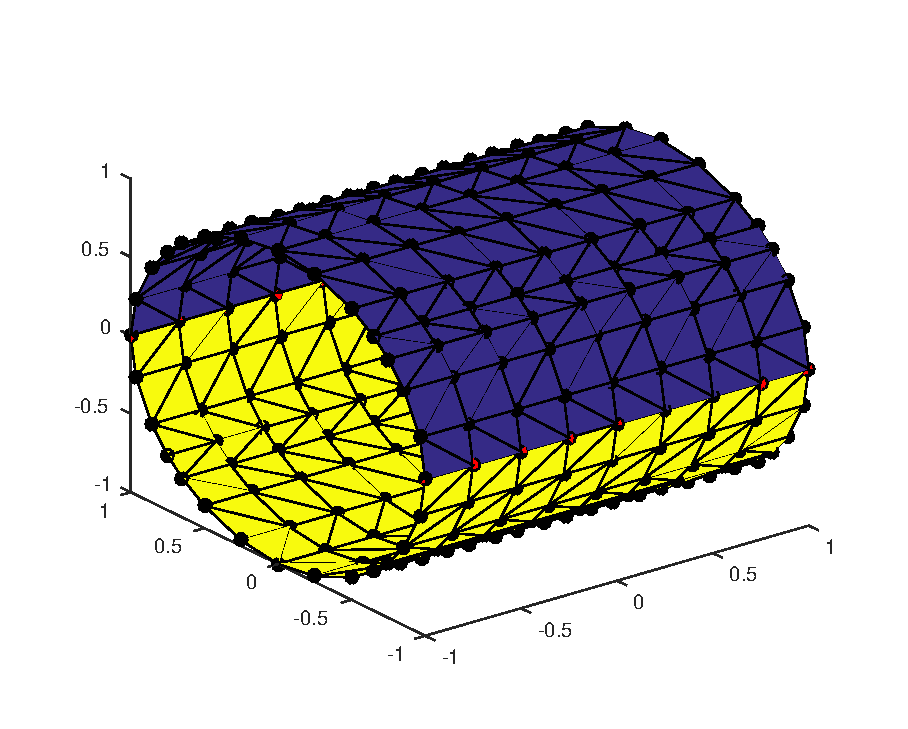
\includegraphics[width=2.9cm]{Pictures/FittingWorkflow/DistriCylinder/distri.eps}}
        node [pos=.5,inner sep=0pt](N3)             
                {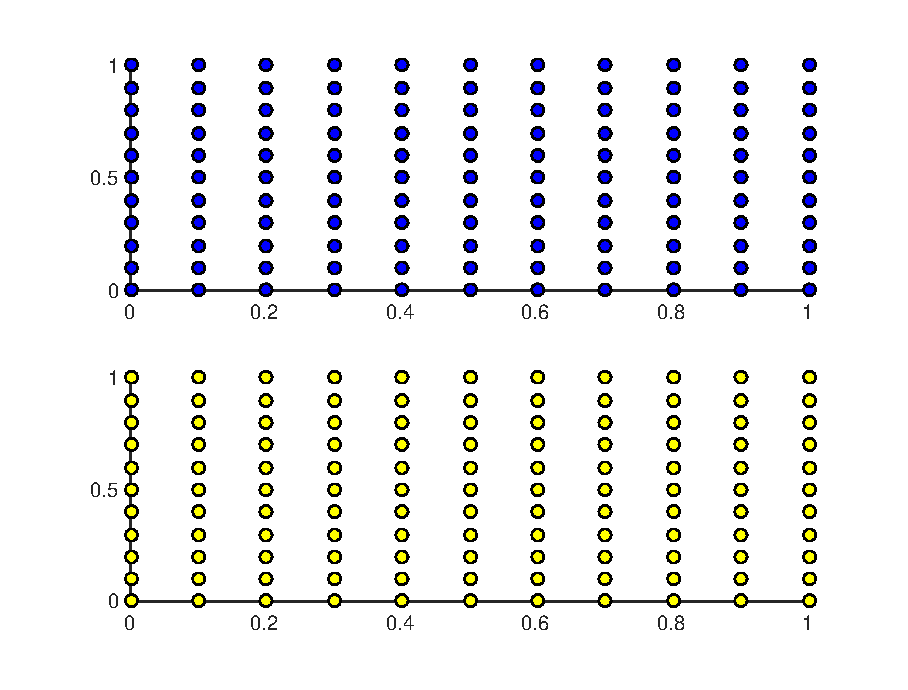
\includegraphics[width=2.9cm]{Pictures/FittingWorkflow/ParameterSpaces/spaces.eps}}
        node [pos=.79,inner sep=0pt](N4) 
                {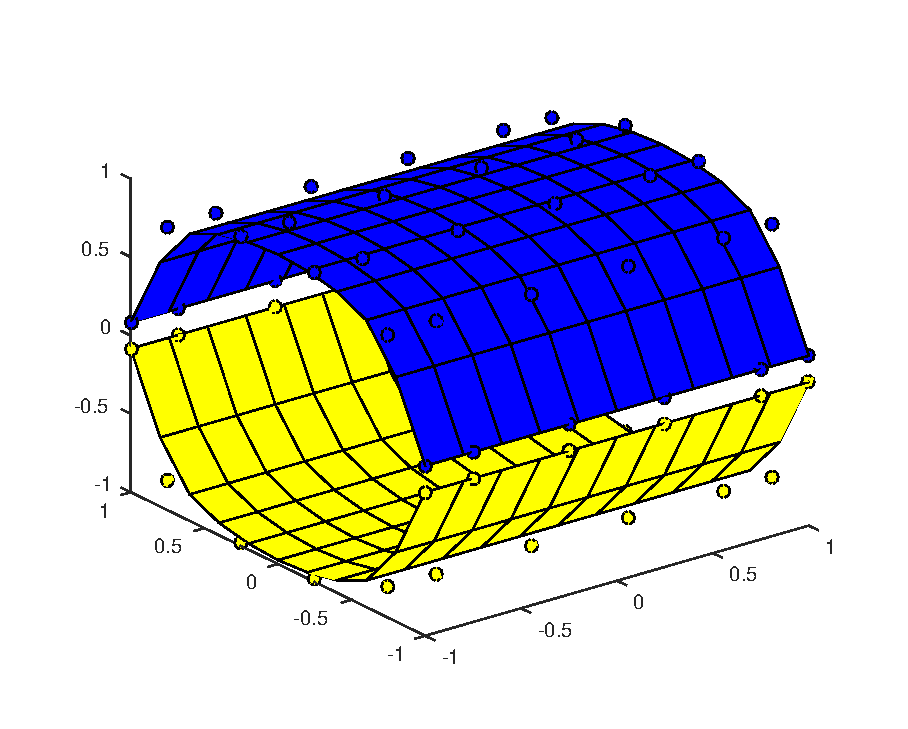
\includegraphics[width=2.9cm]{Pictures/FittingWorkflow/NURBSnotconn/notconn.eps}}
        node [pos=1,inner sep=0pt](N5)
                {\includegraphics[width=2.9cm]{Pictures/FittingWorkflow/PureCylinder/pure.eps}};
        \end{pgfonlayer}
        \draw[thick,->] (N1) -- (N2);
        \draw[thick,->] (N2) -- (N3);
        \draw[thick,->] (N3) -- (N4);
        \draw[thick,->] (N4) -- (N5);                
        \end{tikzpicture}
\end{frame}

\begin{frame}{B--Spline Fitting: Open questions}
\begin{itemize}
\item How to distribute our data into patches?
\item How to parameterize obtained patches?
\item How to connect several patches after fitting?
\end{itemize}
\end{frame}

\begin{frame}{B--Spline Fitting pipeline according to M. Eck\& H. Hoppe}
\begin{figure}
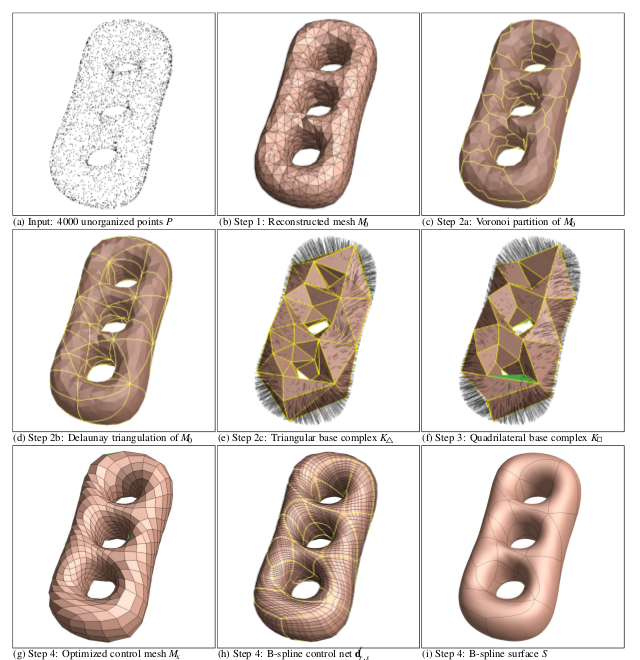
\includegraphics[width=0.625\linewidth]{Pictures/HoppePipeline.png}
\end{figure}
\end{frame}

\begin{frame}{B--Spline Fitting: Parameter correction}
\begin{variableblock}{The task:}{bg=cyan,fg=white}{bg=white,fg=black}
For \textit{fixed} control points $C_{i,j}$, find an optimal parametrization $\left\lbrace u_\alpha,v_\alpha \right\rbrace$.
\end{variableblock}
% This file was created by matlab2tikz.
% Minimal pgfplots version: 1.3
%
%The latest updates can be retrieved from
%  http://www.mathworks.com/matlabcentral/fileexchange/22022-matlab2tikz
%where you can also make suggestions and rate matlab2tikz.
\definecolor{mycolor1}{rgb}{0.00000,0.44700,0.74100}%
\definecolor{mycolor2}{rgb}{0.85000,0.32500,0.09800}%
\definecolor{mycolor3}{rgb}{0.92900,0.69400,0.12500}%
\definecolor{mycolor4}{rgb}{0.49400,0.18400,0.55600}%
\definecolor{mycolor5}{rgb}{0.46600,0.67400,0.18800}%
\definecolor{mycolor6}{rgb}{0.30100,0.74500,0.93300}%
\definecolor{mycolor7}{rgb}{0.63500,0.07800,0.18400}%
%
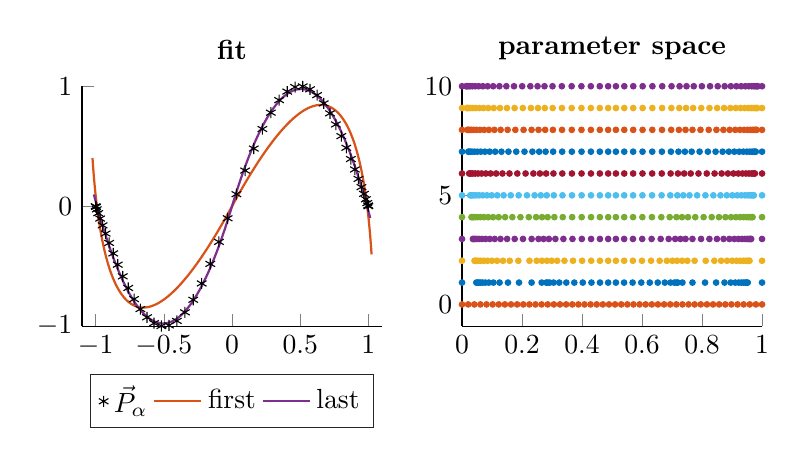
\begin{tikzpicture}

\begin{axis}[%
width=1.5in,
height=1.2in,
at={(1.9in,0in)},
scale only axis,
xmin=0,
xmax=1,
ymin=-1,
ymax=10,
title style={font=\bfseries},
title={parameter space},
axis x line*=bottom,
axis y line*=left
]
\addplot [color=mycolor2,only marks,mark=*,mark options={solid},mark size=1.0,forget plot]
  table[row sep=crcr]{%
0	0\\
0.0204081632653061	0\\
0.0408163265306122	0\\
0.0612244897959184	0\\
0.0816326530612245	0\\
0.102040816326531	0\\
0.122448979591837	0\\
0.142857142857143	0\\
0.163265306122449	0\\
0.183673469387755	0\\
0.204081632653061	0\\
0.224489795918367	0\\
0.244897959183673	0\\
0.26530612244898	0\\
0.285714285714286	0\\
0.306122448979592	0\\
0.326530612244898	0\\
0.346938775510204	0\\
0.36734693877551	0\\
0.387755102040816	0\\
0.408163265306122	0\\
0.428571428571429	0\\
0.448979591836735	0\\
0.469387755102041	0\\
0.489795918367347	0\\
0.510204081632653	0\\
0.530612244897959	0\\
0.551020408163265	0\\
0.571428571428571	0\\
0.591836734693878	0\\
0.612244897959184	0\\
0.63265306122449	0\\
0.653061224489796	0\\
0.673469387755102	0\\
0.693877551020408	0\\
0.714285714285714	0\\
0.73469387755102	0\\
0.755102040816326	0\\
0.775510204081633	0\\
0.795918367346939	0\\
0.816326530612245	0\\
0.836734693877551	0\\
0.857142857142857	0\\
0.877551020408163	0\\
0.897959183673469	0\\
0.918367346938776	0\\
0.938775510204082	0\\
0.959183673469388	0\\
0.979591836734694	0\\
1	0\\
};
\addplot [color=mycolor1,only marks,mark=*,mark options={solid}, mark size=1,forget plot]
  table[row sep=crcr]{%
0	1\\
0.0476838233006445	1\\
0.0516766208949312	1\\
0.0563838628600797	1\\
0.0620622276178283	1\\
0.069072258283093	1\\
0.0779285696239553	1\\
0.0893820271943413	1\\
0.104549394663529	1\\
0.125072882172608	1\\
0.153083855779082	1\\
0.189964842753583	1\\
0.231854096616098	1\\
0.26543408435859	1\\
0.280627749655958	1\\
0.285493191274105	1\\
0.292110703492985	1\\
0.305029289001894	1\\
0.324020085032337	1\\
0.34759048298838	1\\
0.374209772691306	1\\
0.40254135189314	1\\
0.431436032186309	1\\
0.45990322380416	1\\
0.487100039856337	1\\
0.512899960143663	1\\
0.54009677619584	1\\
0.56856396781369	1\\
0.59745864810686	1\\
0.625790227308694	1\\
0.65240951701162	1\\
0.675979914967664	1\\
0.694970710998107	1\\
0.707889296507016	1\\
0.714506808725896	1\\
0.719372250344042	1\\
0.73456591564141	1\\
0.768145903383902	1\\
0.810035157246416	1\\
0.846916144220918	1\\
0.874927117827392	1\\
0.895450605336471	1\\
0.910617972805659	1\\
0.922071430376045	1\\
0.930927741716907	1\\
0.937937772382172	1\\
0.94361613713992	1\\
0.948323379105069	1\\
0.952316176699355	1\\
1	1\\
};
\addplot [color=mycolor3,only marks,mark=*,mark options={solid},mark size=1.0,forget plot]
  table[row sep=crcr]{%
0	2\\
0.0416653560473921	2\\
0.044149304911163	2\\
0.0483983872549571	2\\
0.0544865105496371	2\\
0.0625031016785074	2\\
0.0725599357432915	2\\
0.08480168763338	2\\
0.0994164472770094	2\\
0.116620154914589	2\\
0.136530770160297	2\\
0.159091500217023	2\\
0.187595727441062	2\\
0.22477183243978	2\\
0.248826651811921	2\\
0.266493460365047	2\\
0.283315597980535	2\\
0.298812842503523	2\\
0.317171094582846	2\\
0.341376637400973	2\\
0.369942590302591	2\\
0.40026939929454	2\\
0.430553047977134	2\\
0.459729001401392	2\\
0.487124307875687	2\\
0.512875692124313	2\\
0.540270998598608	2\\
0.569446952022866	2\\
0.59973060070546	2\\
0.63005740969741	2\\
0.658623362599028	2\\
0.682828905417155	2\\
0.701187157496477	2\\
0.716684402019466	2\\
0.733506539634953	2\\
0.751173348188079	2\\
0.775228167560221	2\\
0.812404272558938	2\\
0.840908499782977	2\\
0.863469229839703	2\\
0.883379845085411	2\\
0.90058355272299	2\\
0.91519831236662	2\\
0.927440064256708	2\\
0.937496898321493	2\\
0.945513489450363	2\\
0.951601612745043	2\\
0.955850695088837	2\\
0.958334643952608	2\\
1	2\\
};
\addplot [color=mycolor4,only marks,mark=*,mark options={solid},mark size=1.0,forget plot]
  table[row sep=crcr]{%
0	3\\
0.0362499369160879	3\\
0.0387342090700992	3\\
0.0429187967129508	3\\
0.0488702351484257	3\\
0.0566787249084294	3\\
0.0664554538242147	3\\
0.078330372287793	3\\
0.092452000737119	3\\
0.108992820786758	3\\
0.128168556315213	3\\
0.15027084195055	3\\
0.175492386141122	3\\
0.203239440391906	3\\
0.231976229735242	3\\
0.254878014738801	3\\
0.271856930048874	3\\
0.289467561896589	3\\
0.311154833563384	3\\
0.337866004655871	3\\
0.368105740464445	3\\
0.399412091899167	3\\
0.430203358772746	3\\
0.459618960378752	3\\
0.487109371577258	3\\
0.512890628422742	3\\
0.540381039621248	3\\
0.569796641227254	3\\
0.600587908100833	3\\
0.631894259535555	3\\
0.662133995344129	3\\
0.688845166436617	3\\
0.710532438103412	3\\
0.728143069951126	3\\
0.745121985261199	3\\
0.768023770264758	3\\
0.796760559608094	3\\
0.824507613858878	3\\
0.849729158049449	3\\
0.871831443684787	3\\
0.891007179213242	3\\
0.907547999262881	3\\
0.921669627712207	3\\
0.933544546175785	3\\
0.943321275091571	3\\
0.951129764851574	3\\
0.957081203287049	3\\
0.961265790929901	3\\
0.963750063083912	3\\
1	3\\
};
\addplot [color=mycolor5,only marks,mark=*,mark options={solid},mark size=1.0,forget plot]
  table[row sep=crcr]{%
0	4\\
0.0314228933699868	4\\
0.0338914153131619	4\\
0.0380493053306543	4\\
0.0439600292816213	4\\
0.0517085721209867	4\\
0.0613980543751678	4\\
0.0731462067013899	4\\
0.0870825969412124	4\\
0.103347971494109	4\\
0.122097126287	4\\
0.143503085556731	4\\
0.16773714298968	4\\
0.194722104661774	4\\
0.222609628649386	4\\
0.246888151355787	4\\
0.266689147331003	4\\
0.285352182763485	4\\
0.307779994315681	4\\
0.335798954848373	4\\
0.36703972365524	4\\
0.398886111853062	4\\
0.429949510453948	4\\
0.459509211867207	4\\
0.487081818695471	4\\
0.512918181304529	4\\
0.540490788132793	4\\
0.570050489546052	4\\
0.601113888146938	4\\
0.63296027634476	4\\
0.664201045151627	4\\
0.692220005684319	4\\
0.714647817236515	4\\
0.733310852668997	4\\
0.753111848644213	4\\
0.777390371350614	4\\
0.805277895338226	4\\
0.832262857010319	4\\
0.856496914443269	4\\
0.877902873713	4\\
0.896652028505891	4\\
0.912917403058787	4\\
0.92685379329861	4\\
0.938601945624832	4\\
0.948291427879013	4\\
0.956039970718379	4\\
0.961950694669346	4\\
0.966108584686838	4\\
0.968577106630013	4\\
1	4\\
};
\addplot [color=mycolor6,only marks,mark=*,mark options={solid},mark size=1.0,forget plot]
  table[row sep=crcr]{%
0	5\\
0.0272770065628705	5\\
0.0297407955784723	5\\
0.0338898320501928	5\\
0.0397860305889236	5\\
0.0475118821054528	5\\
0.0571666467960491	5\\
0.0688621136844639	5\\
0.0827186132869548	5\\
0.0988622977850234	5\\
0.117424717551317	5\\
0.138542949792658	5\\
0.162338113622752	5\\
0.18872925175867	5\\
0.216490683487702	5\\
0.241838796731688	5\\
0.262536690022851	5\\
0.282352315681186	5\\
0.305945739121022	5\\
0.334829003042136	5\\
0.366566371841917	5\\
0.398639980785313	5\\
0.429812765990864	5\\
0.459438352181525	5\\
0.487060368010503	5\\
0.512939631989497	5\\
0.540561647818474	5\\
0.570187234009136	5\\
0.601360019214687	5\\
0.633433628158083	5\\
0.665170996957863	5\\
0.694054260878978	5\\
0.717647684318813	5\\
0.737463309977149	5\\
0.758161203268312	5\\
0.783509316512298	5\\
0.81127074824133	5\\
0.837661886377248	5\\
0.861457050207342	5\\
0.882575282448683	5\\
0.901137702214977	5\\
0.917281386713045	5\\
0.931137886315536	5\\
0.942833353203951	5\\
0.952488117894547	5\\
0.960213969411076	5\\
0.966110167949807	5\\
0.970259204421528	5\\
0.972722993437129	5\\
1	5\\
};
\addplot [color=mycolor7,only marks,mark=*,mark options={solid},mark size=1.0,forget plot]
  table[row sep=crcr]{%
0	6\\
0.0237609786558798	6\\
0.0262237276857787	6\\
0.0303704597700029	6\\
0.0362621365657139	6\\
0.0439797035051642	6\\
0.0536200179050556	6\\
0.0652911713134915	6\\
0.0791077785200679	6\\
0.0951870559809116	6\\
0.113646476727846	6\\
0.134601522017932	6\\
0.158146591408174	6\\
0.184214213908735	6\\
0.211848820480999	6\\
0.237790417766162	6\\
0.259575504064539	6\\
0.28023977800151	6\\
0.304665358415746	6\\
0.334214699727315	6\\
0.366268140636599	6\\
0.398467896396581	6\\
0.429703483140367	6\\
0.45937521176289	6\\
0.48703970984863	6\\
0.51296029015137	6\\
0.540624788237109	6\\
0.570296516859632	6\\
0.601532103603419	6\\
0.633731859363401	6\\
0.665785300272684	6\\
0.695334641584254	6\\
0.71976022199849	6\\
0.740424495935461	6\\
0.762209582233838	6\\
0.788151179519001	6\\
0.815785786091265	6\\
0.841853408591826	6\\
0.865398477982068	6\\
0.886353523272154	6\\
0.904812944019088	6\\
0.920892221479932	6\\
0.934708828686508	6\\
0.946379982094944	6\\
0.956020296494836	6\\
0.963737863434286	6\\
0.969629540229997	6\\
0.973776272314221	6\\
0.97623902134412	6\\
1	6\\
};
\addplot [color=mycolor1,only marks,mark=*,mark options={solid},mark size=1.0,forget plot]
  table[row sep=crcr]{%
0	7\\
0.0207733472461017	7\\
0.0232367839696881	7\\
0.0273842775262843	7\\
0.0332761435208299	7\\
0.0409922713795025	7\\
0.0506278652662873	7\\
0.0622884624421414	7\\
0.0760847290266095	7\\
0.0921277393187555	7\\
0.110525394912657	7\\
0.131378733311617	7\\
0.154764410025885	7\\
0.180620565918715	7\\
0.20816189201025	7\\
0.234547905422584	7\\
0.257096129826328	7\\
0.278534019900731	7\\
0.303699536715523	7\\
0.333759506024575	7\\
0.366032660990815	7\\
0.398317596806283	7\\
0.429600854774898	7\\
0.459313551452817	7\\
0.487019116470184	7\\
0.512980883529816	7\\
0.540686448547183	7\\
0.570399145225102	7\\
0.601682403193717	7\\
0.633967339009185	7\\
0.666240493975425	7\\
0.696300463284477	7\\
0.721465980099269	7\\
0.742903870173672	7\\
0.765452094577416	7\\
0.79183810798975	7\\
0.819379434081285	7\\
0.845235589974115	7\\
0.868621266688383	7\\
0.889474605087343	7\\
0.907872260681244	7\\
0.92391527097339	7\\
0.937711537557859	7\\
0.949372134733713	7\\
0.959007728620497	7\\
0.96672385647917	7\\
0.972615722473716	7\\
0.976763216030312	7\\
0.979226652753898	7\\
1	7\\
};
\addplot [color=mycolor2,only marks,mark=*,mark options={solid},mark size=1.0,forget plot]
  table[row sep=crcr]{%
0	8\\
0.0182220411676916	8\\
0.0206870969902833	8\\
0.0248370162762639	8\\
0.0307316524930403	8\\
0.03845013231112	8\\
0.0480864548975427	8\\
0.0597442825669116	8\\
0.0735313712160743	8\\
0.0895542648721145	8\\
0.10791382036412	8\\
0.128700467321675	8\\
0.151977614843374	8\\
0.177684734443693	8\\
0.205147130928488	8\\
0.231841219705446	8\\
0.255033834080893	8\\
0.277118428877168	8\\
0.302903708853299	8\\
0.333373958485919	8\\
0.365816236007663	8\\
0.398170359689846	8\\
0.429497783824412	8\\
0.459251316251577	8\\
0.486998359746791	8\\
0.513001640253209	8\\
0.540748683748423	8\\
0.570502216175588	8\\
0.601829640310154	8\\
0.634183763992336	8\\
0.666626041514081	8\\
0.697096291146701	8\\
0.722881571122832	8\\
0.744966165919106	8\\
0.768158780294554	8\\
0.794852869071512	8\\
0.822315265556307	8\\
0.848022385156627	8\\
0.871299532678325	8\\
0.89208617963588	8\\
0.910445735127886	8\\
0.926468628783926	8\\
0.940255717433088	8\\
0.951913545102457	8\\
0.96154986768888	8\\
0.96926834750696	8\\
0.975162983723736	8\\
0.979312903009717	8\\
0.981777958832308	8\\
1	8\\
};
\addplot [color=mycolor3,only marks,mark=*,mark options={solid},mark size=1.0,forget plot]
  table[row sep=crcr]{%
0	9\\
0.0160320557917812	9\\
0.0184992348376754	9\\
0.0226524944379398	9\\
0.0285513484942449	9\\
0.0362743568785982	9\\
0.0459146136904771	9\\
0.057574360619101	9\\
0.0713591350271706	9\\
0.0873720155414736	9\\
0.105708461923528	9\\
0.126450754726286	9\\
0.149651904874916	9\\
0.175250367924675	9\\
0.202646505175701	9\\
0.229563645128417	9\\
0.253273135906953	9\\
0.275912884186473	9\\
0.302224745917947	9\\
0.333029665390337	9\\
0.365609306820061	9\\
0.398024527987436	9\\
0.429395020791103	9\\
0.459189498499215	9\\
0.486977857449103	9\\
0.513022142550897	9\\
0.540810501500785	9\\
0.570604979208897	9\\
0.601975472012564	9\\
0.634390693179939	9\\
0.666970334609663	9\\
0.697775254082053	9\\
0.724087115813527	9\\
0.746726864093047	9\\
0.770436354871583	9\\
0.797353494824298	9\\
0.824749632075325	9\\
0.850348095125084	9\\
0.873549245273714	9\\
0.894291538076472	9\\
0.912627984458526	9\\
0.928640864972829	9\\
0.942425639380899	9\\
0.954085386309523	9\\
0.963725643121402	9\\
0.971448651505755	9\\
0.97734750556206	9\\
0.981500765162325	9\\
0.983967944208219	9\\
1	9\\
};
\addplot [color=mycolor4,only marks,mark=*,mark options={solid},mark size=1.0,forget plot]
  table[row sep=crcr]{%
0	10\\
0.0141435733369102	10\\
0.0166131255308031	10\\
0.0207701939570212	10\\
0.026674038933194	10\\
0.0344027915825963	10\\
0.0440488530208867	10\\
0.0557133662461396	10\\
0.0695001400684967	10\\
0.0855095396226753	10\\
0.103832784014836	10\\
0.12454571875898	10\\
0.147692961624845	10\\
0.173210727652836	10\\
0.200551668840536	10\\
0.22763144755244	10\\
0.251762360819833	10\\
0.274873690985964	10\\
0.301632602505229	10\\
0.332715083399133	10\\
0.365410428554614	10\\
0.397881654893795	10\\
0.429294342797315	10\\
0.459129268983037	10\\
0.486957998072601	10\\
0.513042001927399	10\\
0.540870731016963	10\\
0.570705657202686	10\\
0.602118345106206	10\\
0.634589571445387	10\\
0.667284916600868	10\\
0.698367397494771	10\\
0.725126309014037	10\\
0.748237639180167	10\\
0.77236855244756	10\\
0.799448331159464	10\\
0.826789272347163	10\\
0.852307038375155	10\\
0.87545428124102	10\\
0.896167215985164	10\\
0.914490460377325	10\\
0.930499859931503	10\\
0.94428663375386	10\\
0.955951146979113	10\\
0.965597208417404	10\\
0.973325961066806	10\\
0.979229806042979	10\\
0.983386874469197	10\\
0.98585642666309	10\\
1	10\\
};
\end{axis}

\begin{axis}[%
width=1.5in,
height=1.2in,
at={(0in,0in)},
scale only axis,
xmin=-1.1,
xmax=1.1,
ymin=-1,
ymax=1,
zmin=-1,
zmax=1,
ztick={\empty},
view={0}{90},
title style={font=\bfseries},
title={fit},
axis x line*=bottom,
axis y line*=left,
axis z line*=left,
legend style={legend columns=-1,draw=white!15!black,at={(.5,-0.2)},anchor=north}
]
\addplot3 [color=black,only marks,mark=asterisk,mark options={solid}]
 table[row sep=crcr] {%
1	1.22464679914735e-16	0\\
0.997945392750336	0.00645469422031125	0\\
0.991790013823246	0.0257895726200411	0\\
0.981559156991065	0.0579012152227707	0\\
0.967294863039029	0.102565535114879	0\\
0.949055747010669	0.15936370867247	0\\
0.926916757346022	0.227585875276051	0\\
0.900968867902419	0.306120752697019	0\\
0.871318704123389	0.393342390896339	0\\
0.838088104891841	0.487008397027433	0\\
0.801413621867957	0.5841866038082	0\\
0.761445958369135	0.681228632630398	0\\
0.718349350097728	0.773808338193523	0\\
0.672300890261317	0.857039986504881	0\\
0.623489801858734	0.925684741400745	0\\
0.57211666012217	0.974444612422557	0\\
0.518392568310525	0.99833108711301	0\\
0.462538290240835	0.993082588618416	0\\
0.404783343122394	0.955592655555454	0\\
0.345365054421308	0.884301695154006	0\\
0.284527586631032	0.779501606559857	0\\
0.222520933956314	0.643506206083195	0\\
0.15959989503338	0.480651805390413	0\\
0.0960230259076819	0.297110653812638	0\\
0.0320515775716553	0.100522931137585	0\\
-0.0320515775716552	-0.100522931137584	0\\
-0.0960230259076818	-0.297110653812638	0\\
-0.159599895033379	-0.480651805390412	0\\
-0.222520933956314	-0.643506206083194	0\\
-0.284527586631032	-0.779501606559857	0\\
-0.345365054421307	-0.884301695154006	0\\
-0.404783343122394	-0.955592655555454	0\\
-0.462538290240835	-0.993082588618416	0\\
-0.518392568310525	-0.998331087113011	0\\
-0.57211666012217	-0.974444612422557	0\\
-0.623489801858733	-0.925684741400745	0\\
-0.672300890261317	-0.857039986504881	0\\
-0.718349350097727	-0.773808338193523	0\\
-0.761445958369134	-0.681228632630399	0\\
-0.801413621867957	-0.5841866038082	0\\
-0.838088104891841	-0.487008397027433	0\\
-0.871318704123389	-0.39334239089634	0\\
-0.900968867902419	-0.30612075269702	0\\
-0.926916757346022	-0.227585875276052	0\\
-0.949055747010669	-0.15936370867247	0\\
-0.967294863039029	-0.102565535114879	0\\
-0.981559156991065	-0.0579012152227707	0\\
-0.991790013823246	-0.0257895726200411	0\\
-0.997945392750336	-0.00645469422031125	0\\
-1	-1.22464679914735e-16	0\\
};
 \addlegendentry{$\vec{P}_\alpha$};

\addplot3 [color=mycolor2,solid,thick]
 table[row sep=crcr] {%
1.02329969709317	-0.40178852510658	0\\
1.02063070789183	-0.356770514900464	0\\
1.01780891045272	-0.312580790046975	0\\
1.01483430477583	-0.269219350546113	0\\
1.01170689086118	-0.226686196397879	0\\
1.00842666870876	-0.184981327602272	0\\
1.00499363831856	-0.144104744159292	0\\
1.0014077996906	-0.104056446068939	0\\
0.997669152824872	-0.064836433331214	0\\
0.993777697721372	-0.026444705946116	0\\
0.989733434380102	0.0111187360863547	0\\
0.985536362801063	0.0478538927661981	0\\
0.981186482984254	0.0837607640934142	0\\
0.976683794929676	0.118839350068003	0\\
0.972028298637329	0.153089650689965	0\\
0.967219994107212	0.186511665959299	0\\
0.962258881339326	0.219105395876006	0\\
0.95714496033367	0.250870840440086	0\\
0.951878231090245	0.281807999651538	0\\
0.946458693609051	0.311916873510363	0\\
0.940886347890087	0.341197462016561	0\\
0.935161193933353	0.369649765170132	0\\
0.92928323173885	0.397273782971075	0\\
0.923252461306578	0.424069515419391	0\\
0.917068882636536	0.45003696251508	0\\
0.910732495728725	0.475176124258141	0\\
0.904243300583144	0.499487000648576	0\\
0.897601297199794	0.522969591686382	0\\
0.890806485578675	0.545623897371562	0\\
0.883858865719786	0.567449917704114	0\\
0.876758437623127	0.58844765268404	0\\
0.8695052012887	0.608617102311337	0\\
0.862099156716503	0.627958266586008	0\\
0.854540303906536	0.646471145508051	0\\
0.8468286428588	0.664155739077467	0\\
0.838964173573294	0.681012047294256	0\\
0.830946896050019	0.697040070158417	0\\
0.822776810288975	0.712239807669951	0\\
0.814453916290161	0.726611259828858	0\\
0.805978214053578	0.740154426635137	0\\
0.797349703579225	0.75286930808879	0\\
0.788568384867103	0.764755904189815	0\\
0.779634257917212	0.775814214938212	0\\
0.770547322729551	0.786044240333983	0\\
0.76130757930412	0.795445980377126	0\\
0.75191502764092	0.804019435067642	0\\
0.742369667739951	0.81176460440553	0\\
0.732671499601212	0.818681488390792	0\\
0.722820523224704	0.824770087023426	0\\
0.712816738610427	0.830030400303432	0\\
0.70266014575838	0.834462428230812	0\\
0.692350744668563	0.838066170805564	0\\
0.681888535340977	0.840841628027689	0\\
0.671273517775622	0.842788799897186	0\\
0.660505691972497	0.843907686414057	0\\
0.649585057931603	0.8441982875783	0\\
0.638511615652939	0.843660603389915	0\\
0.627285365136506	0.842294633848904	0\\
0.615906306382304	0.840100378955265	0\\
0.604374439390332	0.837077838708999	0\\
0.59268976416059	0.833227013110106	0\\
0.58085228069308	0.828547902158585	0\\
0.568861988987799	0.823040505854437	0\\
0.55671888904475	0.816704824197662	0\\
0.544422980863931	0.809540857188259	0\\
0.531974264445342	0.80154860482623	0\\
0.519372739788984	0.792728067111573	0\\
0.506618406894857	0.783079244044288	0\\
0.49371126576296	0.772602135624376	0\\
0.480651316393294	0.761296741851838	0\\
0.467438558785858	0.749163062726671	0\\
0.454072992940653	0.736201098248878	0\\
0.440554618857678	0.722410848418457	0\\
0.426883436536934	0.70779231323541	0\\
0.413059445978421	0.692345492699734	0\\
0.399082647182138	0.676070386811432	0\\
0.384953040148086	0.658966995570502	0\\
0.370670624876264	0.641035318976944	0\\
0.356235401366673	0.62227535703076	0\\
0.341647369619312	0.602687109731948	0\\
0.326906529634182	0.582270577080509	0\\
0.312012881411283	0.561025759076443	0\\
0.296966424950614	0.538952655719749	0\\
0.281767160252175	0.516051267010429	0\\
0.266415087315968	0.492321592948481	0\\
0.25091020614199	0.467763633533905	0\\
0.235252516730244	0.442377388766703	0\\
0.219442019080728	0.416162858646872	0\\
0.203478713193442	0.389120043174415	0\\
0.187362599068387	0.361248942349331	0\\
0.171093676705563	0.332549556171619	0\\
0.154671946104969	0.30302188464128	0\\
0.138097407266606	0.272665927758313	0\\
0.121370060190473	0.24148168552272	0\\
0.104489904876571	0.209469157934499	0\\
0.0874569413248993	0.176628344993651	0\\
0.0702711695354585	0.142959246700175	0\\
0.0529325895082482	0.108461863054073	0\\
0.0354412012432683	0.0731361940553427	0\\
0.017797004740519	0.0369822397039852	0\\
2.22044604925031e-16	4.44089209850063e-16	0\\
-0.0177970047405185	-0.0369822397039842	0\\
-0.0354412012432679	-0.0731361940553417	0\\
-0.0529325895082477	-0.108461863054072	0\\
-0.070271169535458	-0.142959246700174	0\\
-0.0874569413248988	-0.176628344993649	0\\
-0.104489904876571	-0.209469157934498	0\\
-0.121370060190472	-0.241481685522718	0\\
-0.138097407266605	-0.272665927758313	0\\
-0.154671946104968	-0.303021884641278	0\\
-0.171093676705563	-0.332549556171618	0\\
-0.187362599068387	-0.361248942349329	0\\
-0.203478713193442	-0.389120043174415	0\\
-0.219442019080727	-0.416162858646871	0\\
-0.235252516730243	-0.442377388766702	0\\
-0.25091020614199	-0.467763633533904	0\\
-0.266415087315967	-0.49232159294848	0\\
-0.281767160252175	-0.516051267010428	0\\
-0.296966424950613	-0.538952655719749	0\\
-0.312012881411282	-0.561025759076442	0\\
-0.326906529634182	-0.582270577080508	0\\
-0.341647369619312	-0.602687109731948	0\\
-0.356235401366672	-0.622275357030759	0\\
-0.370670624876263	-0.641035318976943	0\\
-0.384953040148085	-0.658966995570501	0\\
-0.399082647182137	-0.676070386811431	0\\
-0.413059445978421	-0.692345492699733	0\\
-0.426883436536934	-0.707792313235409	0\\
-0.440554618857678	-0.722410848418457	0\\
-0.454072992940653	-0.736201098248877	0\\
-0.467438558785857	-0.749163062726671	0\\
-0.480651316393293	-0.761296741851837	0\\
-0.493711265762959	-0.772602135624376	0\\
-0.506618406894856	-0.783079244044288	0\\
-0.519372739788984	-0.792728067111572	0\\
-0.531974264445342	-0.801548604826229	0\\
-0.54442298086393	-0.809540857188259	0\\
-0.556718889044749	-0.816704824197661	0\\
-0.568861988987799	-0.823040505854436	0\\
-0.580852280693079	-0.828547902158584	0\\
-0.59268976416059	-0.833227013110105	0\\
-0.604374439390332	-0.837077838708998	0\\
-0.615906306382303	-0.840100378955264	0\\
-0.627285365136506	-0.842294633848903	0\\
-0.638511615652939	-0.843660603389915	0\\
-0.649585057931602	-0.844198287578299	0\\
-0.660505691972497	-0.843907686414056	0\\
-0.671273517775621	-0.842788799897186	0\\
-0.681888535340977	-0.840841628027688	0\\
-0.692350744668563	-0.838066170805563	0\\
-0.702660145758379	-0.834462428230811	0\\
-0.712816738610426	-0.830030400303432	0\\
-0.722820523224704	-0.824770087023425	0\\
-0.732671499601212	-0.818681488390791	0\\
-0.742369667739951	-0.81176460440553	0\\
-0.75191502764092	-0.804019435067641	0\\
-0.76130757930412	-0.795445980377125	0\\
-0.77054732272955	-0.786044240333982	0\\
-0.779634257917211	-0.775814214938211	0\\
-0.788568384867103	-0.764755904189814	0\\
-0.797349703579225	-0.752869308088789	0\\
-0.805978214053577	-0.740154426635137	0\\
-0.814453916290161	-0.726611259828857	0\\
-0.822776810288974	-0.712239807669951	0\\
-0.830946896050019	-0.697040070158416	0\\
-0.838964173573294	-0.681012047294255	0\\
-0.846828642858799	-0.664155739077467	0\\
-0.854540303906535	-0.646471145508051	0\\
-0.862099156716502	-0.627958266586007	0\\
-0.869505201288699	-0.608617102311337	0\\
-0.876758437623127	-0.588447652684039	0\\
-0.883858865719785	-0.567449917704114	0\\
-0.890806485578674	-0.545623897371562	0\\
-0.897601297199794	-0.522969591686382	0\\
-0.904243300583144	-0.499487000648575	0\\
-0.910732495728724	-0.475176124258141	0\\
-0.917068882636536	-0.450036962515079	0\\
-0.923252461306577	-0.424069515419391	0\\
-0.92928323173885	-0.397273782971075	0\\
-0.935161193933353	-0.369649765170131	0\\
-0.940886347890086	-0.341197462016561	0\\
-0.94645869360905	-0.311916873510363	0\\
-0.951878231090244	-0.281807999651538	0\\
-0.95714496033367	-0.250870840440085	0\\
-0.962258881339325	-0.219105395876005	0\\
-0.967219994107211	-0.186511665959298	0\\
-0.972028298637328	-0.153089650689965	0\\
-0.976683794929676	-0.118839350068002	0\\
-0.981186482984254	-0.0837607640934143	0\\
-0.985536362801062	-0.0478538927661981	0\\
-0.989733434380101	-0.0111187360863548	0\\
-0.993777697721371	0.026444705946116	0\\
-0.997669152824871	0.0648364333312139	0\\
-1.0014077996906	0.104056446068939	0\\
-1.00499363831856	0.144104744159292	0\\
-1.00842666870876	0.184981327602272	0\\
-1.01170689086118	0.226686196397879	0\\
-1.01483430477583	0.269219350546113	0\\
-1.01780891045271	0.312580790046975	0\\
-1.02063070789183	0.356770514900464	0\\
-1.02329969709317	0.40178852510658	0\\
};
 \addlegendentry{first};

\addplot3 [color=mycolor4,thick]
 table[row sep=crcr] {%
1.01343438005398	-0.0982276622577756	0\\
1.00373946063245	-0.0566450550122122	0\\
0.994035663950736	-0.015882656466103	0\\
0.984322990008839	0.0240595333805519	0\\
0.97460143880676	0.0631815145277525	0\\
0.964871010344499	0.101483286975499	0\\
0.955131704622056	0.138964850723791	0\\
0.945383521639432	0.175626205772629	0\\
0.935626461396625	0.211467352122013	0\\
0.925860523893636	0.246488289771942	0\\
0.916085709130466	0.280689018722417	0\\
0.906302017107113	0.314069538973438	0\\
0.896509447823578	0.346629850525005	0\\
0.886708001279862	0.378369953377117	0\\
0.876897677475963	0.409289847529775	0\\
0.867078476411883	0.439389532982979	0\\
0.85725039808762	0.468669009736728	0\\
0.847413442503176	0.497128277791024	0\\
0.83756760965855	0.524767337145865	0\\
0.827712899553742	0.551586187801252	0\\
0.817849312188752	0.577584829757184	0\\
0.807976847563579	0.602763263013663	0\\
0.798095505678225	0.627121487570687	0\\
0.788205286532689	0.650659503428257	0\\
0.778306190126971	0.673377310586372	0\\
0.768398216461071	0.695274909045033	0\\
0.758481365534989	0.71635229880424	0\\
0.748555637348725	0.736609479863993	0\\
0.73862103190228	0.756046452224292	0\\
0.728677549195652	0.774663215885136	0\\
0.718725189228842	0.792459770846526	0\\
0.70876395200185	0.809436117108462	0\\
0.698793837514677	0.825592254670943	0\\
0.688814845767321	0.84092818353397	0\\
0.678826976759783	0.855443903697543	0\\
0.668830230492064	0.869139415161662	0\\
0.658824606964162	0.882014717926327	0\\
0.648810106176079	0.894069811991537	0\\
0.638786728127814	0.905304697357293	0\\
0.628754472819366	0.915719374023594	0\\
0.618713340250737	0.925313841990442	0\\
0.608663330421926	0.934088101257835	0\\
0.598604443332933	0.942042151825774	0\\
0.588536678983757	0.949175993694259	0\\
0.5784600373744	0.955489626863289	0\\
0.568374518504861	0.960983051332865	0\\
0.55828012237514	0.965656267102987	0\\
0.548176848985237	0.969509274173655	0\\
0.538064698335152	0.972542072544868	0\\
0.527943670424885	0.974754662216627	0\\
0.517813765254436	0.976147043188932	0\\
0.507674982823805	0.976719215461783	0\\
0.497527323132993	0.976471179035179	0\\
0.487370786181998	0.975402933909121	0\\
0.477205371970821	0.973514480083609	0\\
0.467031080499463	0.970805817558643	0\\
0.456847911767922	0.967276946334222	0\\
0.4466558657762	0.962927866410347	0\\
0.436454942524295	0.957758577787018	0\\
0.426245142012209	0.951769080464235	0\\
0.41602646423994	0.944959374441997	0\\
0.40579890920749	0.937329459720305	0\\
0.395562476914858	0.928879336299159	0\\
0.385317167362043	0.919609004178559	0\\
0.375062980549047	0.909518463358504	0\\
0.364799916475869	0.898607713838995	0\\
0.354527975142509	0.886876755620032	0\\
0.344247156548967	0.874325588701614	0\\
0.333957460695242	0.860954213083742	0\\
0.323658887581336	0.846762628766417	0\\
0.313351437207248	0.831750835749636	0\\
0.303035109572979	0.815918834033402	0\\
0.292709904678527	0.799266623617713	0\\
0.282375822523893	0.78179420450257	0\\
0.272032863109077	0.763501576687973	0\\
0.261681026434079	0.744388740173921	0\\
0.2513203124989	0.724455694960415	0\\
0.240950721303538	0.703702441047456	0\\
0.230572252847994	0.682128978435041	0\\
0.220184907132269	0.659735307123173	0\\
0.209788684156361	0.63652142711185	0\\
0.199383583920272	0.612487338401073	0\\
0.188969606424	0.587633040990841	0\\
0.178546751667547	0.561958534881156	0\\
0.168115019650912	0.535463820072016	0\\
0.157674410374094	0.508148896563422	0\\
0.147224923837095	0.480013764355374	0\\
0.136766560039914	0.451058423447871	0\\
0.126299318982551	0.421282873840915	0\\
0.115823200665006	0.390687115534504	0\\
0.105338205087279	0.359271148528638	0\\
0.0948443322493695	0.327034972823319	0\\
0.0843415821512786	0.293978588418545	0\\
0.0738299547930055	0.260101995314316	0\\
0.0633094501745507	0.225405193510634	0\\
0.0527800682959139	0.189888183007497	0\\
0.0422418091570951	0.153550963804907	0\\
0.0316946727580944	0.116393535902862	0\\
0.0211386590989117	0.0784158993013623	0\\
0.010573768179547	0.0396180540004087	0\\
3.33066907387547e-16	6.66133814775094e-16	0\\
-0.0105737681795463	-0.0396180540004074	0\\
-0.021138659098911	-0.0784158993013611	0\\
-0.0316946727580937	-0.116393535902861	0\\
-0.0422418091570945	-0.153550963804905	0\\
-0.0527800682959131	-0.189888183007496	0\\
-0.0633094501745501	-0.225405193510633	0\\
-0.0738299547930048	-0.260101995314315	0\\
-0.084341582151278	-0.293978588418543	0\\
-0.0948443322493688	-0.327034972823317	0\\
-0.105338205087278	-0.359271148528637	0\\
-0.115823200665005	-0.390687115534502	0\\
-0.12629931898255	-0.421282873840913	0\\
-0.136766560039913	-0.45105842344787	0\\
-0.147224923837095	-0.480013764355373	0\\
-0.157674410374094	-0.508148896563421	0\\
-0.168115019650911	-0.535463820072015	0\\
-0.178546751667546	-0.561958534881155	0\\
-0.188969606424	-0.58763304099084	0\\
-0.199383583920271	-0.612487338401071	0\\
-0.209788684156361	-0.636521427111848	0\\
-0.220184907132268	-0.659735307123172	0\\
-0.230572252847994	-0.68212897843504	0\\
-0.240950721303537	-0.703702441047454	0\\
-0.251320312498899	-0.724455694960414	0\\
-0.261681026434079	-0.74438874017392	0\\
-0.272032863109077	-0.763501576687972	0\\
-0.282375822523892	-0.781794204502569	0\\
-0.292709904678526	-0.799266623617712	0\\
-0.303035109572978	-0.815918834033401	0\\
-0.313351437207248	-0.831750835749635	0\\
-0.323658887581336	-0.846762628766415	0\\
-0.333957460695242	-0.860954213083741	0\\
-0.344247156548966	-0.874325588701613	0\\
-0.354527975142508	-0.88687675562003	0\\
-0.364799916475868	-0.898607713838994	0\\
-0.375062980549046	-0.909518463358502	0\\
-0.385317167362043	-0.919609004178557	0\\
-0.395562476914857	-0.928879336299158	0\\
-0.405798909207489	-0.937329459720304	0\\
-0.416026464239939	-0.944959374441996	0\\
-0.426245142012208	-0.951769080464234	0\\
-0.436454942524294	-0.957758577787017	0\\
-0.446655865776199	-0.962927866410346	0\\
-0.456847911767921	-0.967276946334221	0\\
-0.467031080499462	-0.970805817558642	0\\
-0.477205371970821	-0.973514480083608	0\\
-0.487370786181997	-0.97540293390912	0\\
-0.497527323132992	-0.976471179035178	0\\
-0.507674982823805	-0.976719215461782	0\\
-0.517813765254436	-0.976147043188931	0\\
-0.527943670424885	-0.974754662216627	0\\
-0.538064698335152	-0.972542072544867	0\\
-0.548176848985237	-0.969509274173654	0\\
-0.55828012237514	-0.965656267102986	0\\
-0.568374518504861	-0.960983051332864	0\\
-0.5784600373744	-0.955489626863288	0\\
-0.588536678983757	-0.949175993694257	0\\
-0.598604443332932	-0.942042151825773	0\\
-0.608663330421925	-0.934088101257834	0\\
-0.618713340250737	-0.925313841990441	0\\
-0.628754472819366	-0.915719374023593	0\\
-0.638786728127813	-0.905304697357292	0\\
-0.648810106176078	-0.894069811991536	0\\
-0.658824606964162	-0.882014717926326	0\\
-0.668830230492063	-0.869139415161661	0\\
-0.678826976759783	-0.855443903697543	0\\
-0.688814845767321	-0.84092818353397	0\\
-0.698793837514676	-0.825592254670942	0\\
-0.70876395200185	-0.809436117108461	0\\
-0.718725189228842	-0.792459770846525	0\\
-0.728677549195651	-0.774663215885135	0\\
-0.738621031902279	-0.756046452224291	0\\
-0.748555637348725	-0.736609479863993	0\\
-0.758481365534989	-0.71635229880424	0\\
-0.768398216461071	-0.695274909045033	0\\
-0.778306190126971	-0.673377310586371	0\\
-0.788205286532689	-0.650659503428256	0\\
-0.798095505678225	-0.627121487570686	0\\
-0.807976847563579	-0.602763263013662	0\\
-0.817849312188751	-0.577584829757184	0\\
-0.827712899553742	-0.551586187801251	0\\
-0.83756760965855	-0.524767337145864	0\\
-0.847413442503176	-0.497128277791023	0\\
-0.85725039808762	-0.468669009736728	0\\
-0.867078476411883	-0.439389532982978	0\\
-0.876897677475963	-0.409289847529775	0\\
-0.886708001279862	-0.378369953377116	0\\
-0.896509447823578	-0.346629850525005	0\\
-0.906302017107113	-0.314069538973438	0\\
-0.916085709130465	-0.280689018722417	0\\
-0.925860523893636	-0.246488289771942	0\\
-0.935626461396625	-0.211467352122013	0\\
-0.945383521639431	-0.175626205772629	0\\
-0.955131704622056	-0.138964850723791	0\\
-0.964871010344499	-0.101483286975499	0\\
-0.97460143880676	-0.0631815145277527	0\\
-0.984322990008839	-0.0240595333805521	0\\
-0.994035663950736	0.0158826564661028	0\\
-1.00373946063245	0.056645055012212	0\\
-1.01343438005398	0.0982276622577754	0\\
};
 \addlegendentry{last};

\end{axis}
\end{tikzpicture}%

\end{frame}

\begin{frame}{Summary}
\begin{variableblock}{What's done?}{bg=cyan,fg=white}{bg=white,fg=black}
\begin{itemize}
\item first part of the pipeline from CAD model to optimized voxel model
\item identified crucial points in the fitting problem
\end{itemize}
\end{variableblock}
\end{frame}

\begin{frame}{Outlook}
\begin{variableblock}{What's next?}{bg=cyan,fg=white}{bg=white,fg=black}
\begin{itemize}
\item further work on M.Eck \& H.Hoppe paper
\item search for algorithm which considers voxel geometry
\end{itemize}
\end{variableblock}
\end{frame}